\documentclass{standalone}
\usepackage[svgnames]{xcolor}
\usepackage{tikz}
\usetikzlibrary{matrix, positioning, arrows.meta}
\tikzset{>=Latex, Blue Box/.style={fill=RoyalBlue, text=white}, Red Box/.style={fill=FireBrick, text=white}, Data Property/.style={matrix of nodes, nodes={draw, minimum width=4ex, minimum height=4ex, anchor=center}, column sep=-0.4pt} }
\begin{document} 
\sffamily \bfseries 
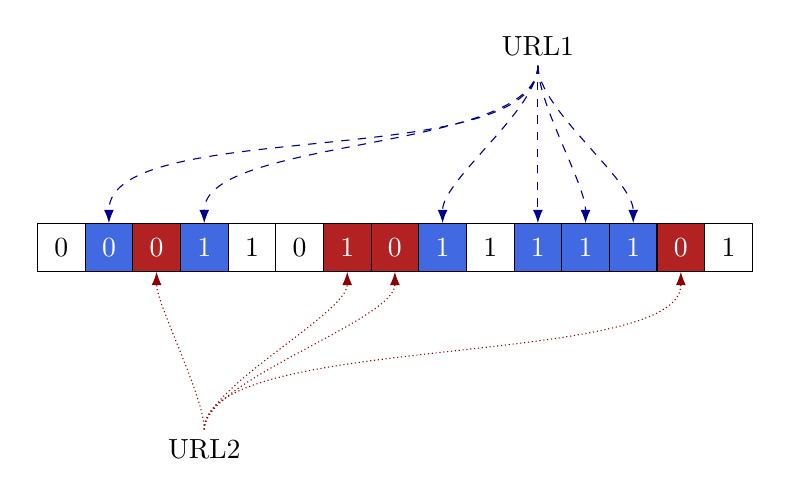
\begin{tikzpicture}
\matrix[Data Property] (Data) {
0 &
|[Blue Box] (R1) | 0 &
|[Red  Box] (M1) | 0 &
|[Blue Box] (R2) | 1 &
1 &
0 &
|[Red  Box] (M2) | 1 &
|[Red  Box] (M3) | 0 &
|[Blue Box] (R3) | 1 &
1 &
|[Blue Box] (R4) | 1 &
|[Blue Box] (R5) | 1 &
|[Blue Box] (R6) | 1 &
|[Red  Box] (M4) | 0 &
1 \\
};
\node[above =2cm of R4] (U1) {URL1}; 
\foreach \x in {1,...,6} {\draw[dashed,->, DarkBlue] (U1) to[out=-90, in=90, looseness=0.6] (R\x);}
\node[below =2cm of R2] (U2) {URL2};
\foreach \x in {1,...,4} {\draw[DarkRed, densely dotted, ->] (U2) to[out=90, in=-90, looseness=0.5] (M\x);}
\end{tikzpicture}
\end{document}